

\documentclass[runningheads]{llncs}
\usepackage[
backend=biber,
style=ieee]{biblatex}
\usepackage{tabularx}
\usepackage{graphicx}
\usepackage{listings}
\usepackage[super]{nth}
\usepackage{caption}
\usepackage{multirow}
\usepackage{hhline}
\usepackage{hyperref}
\graphicspath{ {./images/} }


\usepackage[scaled=.92]{mathptmx}
\usepackage{microtype}
\usepackage{graphicx}
\usepackage{wrapfig}
\usepackage{enumitem}
\usepackage{enumerate}
\usepackage{fancyhdr}
\usepackage{amsmath}
\usepackage{index}
\usepackage{istgame}
\usepackage{multicol}

\usepackage{graphicx}
\addbibresource{refs.bib}
\begin{document}
%
\title{Negation Cue Detection using SVM and XGBoost Classifiers}
%
%\titlerunning{Abbreviated paper title}
% If the paper title is too long for the running head, you can set
% an abbreviated paper title here
%
\author{
Sergio A. Gutierrez Maury (2647606)
}
\authorrunning{Gutierrez Maury S.A}
%
% First names are abbreviated in the running head.
% If there are more than two authors, 'et al.' is used.
%
\institute{Vrije Universiteit Amsterdam}
%
\maketitle              % typeset the header of the contribution

\begin{abstract}

This paper presents a comparative study of two machine learning models, Support Vector Machines (SVM) and XGBoost, for detecting negation cues in text data. Negation cues can significantly impact the meaning of a sentence, and their accurate detection is crucial for obtaining reliable insights from text data. The study evaluates the performance of the models in detecting negation cues and their scope using an ablation analysis. The results show that both SVM and XGBoost models perform well in detecting negation cues, with SVM slightly outperforming XGBoost. The findings of this study can aid in the development of more accurate natural language processing tools for text data analysis. However, the limitations of the study, such as the imbalanced dataset, suggest the need for further research in this area.

\keywords{Support Vector Machine (SVM)  \and XGBoost \and Negation Cue Detection.}
\end{abstract}


\section*{Introduction}
Negation Cue Detection is an essential aspect of Natural Language Processing (NLP) and Text Mining that enables automated systems to classify the sentiment or opinion expressed in a sentence. In essence, negation cues are linguistic markers that indicate the presence of negation in a sentence. They can manifest in diverse forms, such as single words like "never," multi-words like "no longer" and "by no means," or affixes like "im-" and "-less." Negation cues can also be complex, discontinuous, and have a scope that encompasses all negated concepts and events, excluding the negation cue itself \cite{jbara-2012}. 
\\

However, identifying negation cues presents several challenges in NLP and Text Mining. For example, negation cues can have different meanings depending on the context in which they appear, and detecting their scope can be difficult in complex sentences. Moreover, the incorrect detection or omission of negation cues can significantly impact the overall interpretation of the text, leading to unreliable insights and results.
\\

Therefore, accurately detecting negation cues is vital for many NLP and Text Mining tasks, such as Sentiment Analysis \cite{cruz2016machine} and Clinical Text Mining \cite{mehrabi2015deepen}, as it enables automated systems to extract the correct sentiment or opinion expressed in the text data. 
\\

This paper presents two models for automatic negation cue classification,  Support Vector Machines (SVM) and XGBoost, and conduct an ablation study to determine the impact of the features used in automatic detection. The study aims to assess the performance of the models in accurately detecting negation cues and their scope, which is crucial for obtaining reliable insights from text data.
\\

 The paper is structured as follows: firstly, related work in negation cue detection is reviewed. Secondly, an annotation experiment is carried out to gain a deeper knowledge in the data annotation process. Thirdly, a description of the data used in the experiments is presented. Next, the corpus pre-processing and feature extraction is described. After this, the description of the experimental setup is presented, where an ablation study is done, with its results. In section \ref{sec:error}, an error analysis is performed, with the best-performing iteration out of the ablation study, on the circle test set. Finally, the conclusions of the present research are carried out, with the main challenges and limitations discussed.


\section*{Related Work}
Negation Cue detection received a lot of attention from the scientific community \cite{story2020}. For instance, Lapponi et al. (2012) \cite{lapponi2012uio} describe a system submitted by the University of Oslo to the 2012 SEM Shared Task on revolving negation. The authors based their identification of negation cues work on the light-weight classification scheme presented by Velldal et al. (2012) \cite{velldal2012speculation}, using an SVM classifier trained using simple n-gram features over words, both full forms and lemmas of the word in question and of words to the left and to the right of it.
\\

The authors added features to identify morphological or affixal cues in addition to token-level features. The first of these features records character n-grams from both the beginning and end of the base that an affix attaches to (up to five positions). The second feature targets affix cues. The authors try to emulate the effect of a lexicon look-up on the remaining substring after "subtracting" the affix, checking the status of both the remaining substring and its POS tag. 


\begin{table}[!h]
\centering
\caption{\label{tab:chowdhury} Feature set in Chowdhury et al. Negation Cue Classifier}
\begin{tabular}{ll}
\hline
Feature Name & Description \\ \hline
$POS_{i}$ & Part-of-Speech of $token_{i}$ \\
$Lemma_{i}$ & Lemma form of $token_{i}$ \\
$Lemma_{i-1}$ & Lemma form of $token_{i-1}$ \\
$hasNegPrefix$ & \begin{tabular}[c]{@{}l@{}}If $token_{i}$ has a negation prefix and is found \\ inside the automatically created vocabulary \end{tabular} \\
$hasNegSuffix$ & \begin{tabular}[c]{@{}l@{}}If $token_{i}$ has a negation suffix and is found \\ inside the automatically created vocabulary \end{tabular} \\
\textit{matchesNegExp} & If $token_{i}$ is found in \texit{NegExpList} \\

\hline
\end{tabular}
\end{table}

The authors explain the motivation behind this feature as "\textit{the occurrence of a substring such as 'un' in a token such as 'underlying' should be considered more unlikely to be a cue given that the first part of the remaining string (e.g., 'derly') would be an unlikely way to begin a word.}"

Chowdhury et al. (2012) \cite{chowdhury2012fbk} presents a system for the automatic detection of negation cues along with their scopes and corresponding negated events presented for Task 1 of the 2012 SEM Shared Task. The authors claim their approach uses comparatively fewer features than other works developed for the same task. They approach the problem as a sequence classification task, training different 1st order Conditional Random Field classifiers for each of the different sub-tasks. 
For the negation cue detection subtask, the authors automatically collect a vocabulary of all the positive tokens after excluding negation cue affixes from the training data and use them to extract features that could help to identify negation cues that are subtokens. They also create a list of highly probable negation expressions (\textit{NegExpList}) from the training data based on the frequencies. The list contains the following terms: \textit{nor, neither, without, nobody, none, nothing, never, not, no, nowhere} and  \textit{non}. Additional post-processing is done to annotate some obvious negations missed by the classifier. The final feature set for the negation cue classifier is shown in Table \ref{tab:chowdhury}

The extraction of dependency graphs and features based on this could help in modeling the syntactic relationship between each token and the closest negation cue. Jiménez-Zafra et al. (2020) \cite{jimenez2020detecting} focused their work on the detection of negation scopes and cues in Spanish, and among other features, they extracted dependency features as the dependency relation and direction between the token and the cue, and the dependency shortest path from the token in focus to the cue and vice versa. Also, Cruz et al. (2016) \cite{cruz2016machine} showed that highly accurate extraction of syntactic structure is beneficial for the negation scope detection task. Lapponi et al. (2012) \cite{lapponi2012uio} uses features defined over dependency graphs. All these works have in common the use of dependency-based features for the task of Negation Scope and Cue detection, and they have proved that the use of these types of features improves the performance of the classifiers in these tasks.

No mention was found of using the XGBoost algorithm for negation cue detection for English corpora, yet Domınguez-Mas et al. (2019) \cite{xgb2019} applied it and SVM-linear model for the Spanish dataset for negation cue detection, and it performed better than the SVM-linear model. Current research, therefore, aims to compare the performance of these two algorithms for negation cue detection in English.
\section*{Data Annotation Experiment}
This section presents an inter-annotator agreement (IAA) section that aims to gain a better understanding of the annotation process of negation cues in texts related to the vaccination debate using the e-Host annotation tool. The purpose of this section is to compare, analyze, and quantify the annotations made by different annotators and to identify sources of disagreement among them, with the ultimate goal of improving the final classification.

To ensure consistency, the annotation process follows the guidelines provided by Morante et al. \cite{morante2011annotation}. Each member of the group independently annotates the same corpus of texts, which contains a mix of pro and anti-vaccination opinions from various sources, including official sources such as the National Health Service UK, as well as independent publications like the National Vaccine Information Center and Natural News.

The annotation guidelines provide possible negation cues for each part of speech and offer examples on how to determine the scope of the negation. They also include instructions on how to separate the negation scope from the rest of the phrase based on a simple grammatical analysis, which involves reformulating the phrase to test whether a part of it belongs to the scope or not. Specific rules on the separation of scope based on the part of speech that was negated are provided to minimize the annotator's bias. Special constructions such as questions and imperatives are also included in the guidelines, as well as examples of false negations and non-existing scope, to avoid expected mistakes.

Overall, this section aims to provide insights into the annotation process of negation cues and how it could impact the final classification. By comparing, analyzing, and quantifying the annotations made by different annotators, this section contributes to the understanding of the sources of disagreement and helps identify areas for improvement in the annotation process.
% All annotations were added to our \href{https://github.com/Sergi095/Applied-Text-Mining-VU-Course-2023-}{GitHub Repository}

\subsection*{Inter-Annotator Agreement Analysis}
As part of our investigation into the annotation process and its impact on the final classification, an inter-annotator agreement (IAA) analysis was conducted. In this section, we present the results of the IAA analysis and discuss the sources of disagreement among the annotators.

Each member of the group independently annotated a set of 12 texts following the guidelines provided by Morante et al. \cite{morante2011annotation}, which offered detailed instructions on how to identify negation cues and determine their scope. The purpose of the IAA analysis was to compare, analyze, and quantify the annotations made by different annotators and to identify sources of disagreement among them.

\begin{figure}[!h]
\begin{center}
  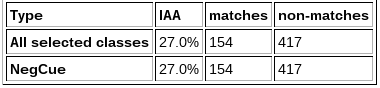
\includegraphics[width=0.6\textwidth]{Plots and results/4way.png}
  \caption{4-way IAA result}
  \label{fig:4way}
\end{center}  
\end{figure}

The results of the IAA analysis were obtained by comparing the annotations made by each member of the group. Figure \ref{fig:Pairwise agreement} shows the pair-wise agreement scores obtained from the analysis. We conducted an error analysis to systematically identify and explain the sources of disagreement among annotators. The analysis was based on a random sample of errors, and patterns were identified and illustrated with examples.

\begin{figure}[!h]
  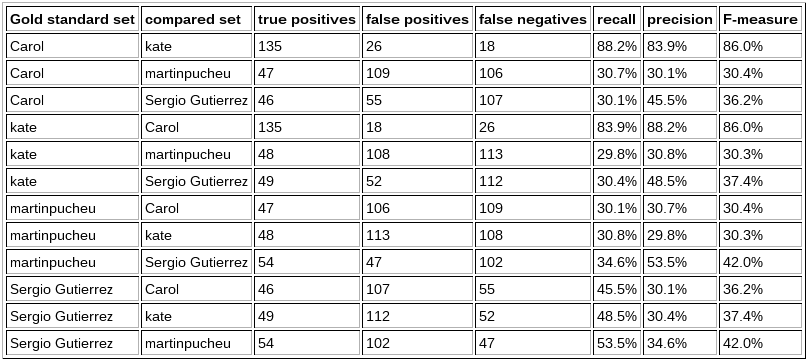
\includegraphics[width=\linewidth]{Plots and results/pairwise.png}
  \caption{Pair-wise agreement}
  \label{fig:Pairwise agreement}
\end{figure}

The results of the analysis revealed that human error and a lack of alignment between the text versions used for annotation were the main sources of disagreements among annotators. Specifically, disagreements arose when annotators failed to highlight the entire word or phrase, instead only highlighting part of it. For example, with words like "unclear", "unprotected", and "unpublished", some annotators highlighted the complete word, while others only highlighted the prefix "un". Similarly, with the word "don't", some annotators only highlighted the contraction, while others did the complete word.

To address these sources of disagreement, we suggest implementing a more thorough training process for the annotators, which could include a detailed review of the guidelines and examples, as well as further practice sessions. Moreover, we suggest that the guidelines could be further expanded to cover more examples of negation cues in different contexts to reduce ambiguity. Additionally, post-processing the annotations to annotate some obvious negations missed by the classifier would also help to improve the overall agreement scores, as shown in Figure \ref{fig:4way}.


To sum up, this section provided insights into the annotation process of negation cues. The inter-annotator agreement analysis helped to identify the sources of disagreement among the annotators and highlighted the need for more thorough training to reduce ambiguity. The results also emphasized the importance of post-processing the annotations to improve the overall agreement scores.

\section*{Methods}
% 




\subsubsection{Support Machine Vectors}
 SVM was first introduced by Vapnik and Cortes(1995) \cite{vapnik1995}, and was quickly recognized as one of the most successful classification algorithms. The basic idea behind the model is finding such a hyperplane between the plotted classes in a way, where the margin, i.e. the distance, between the two classes is maximized. SVM algorithms show great robustness against noise and control over-fitting \cite{robust2009}. Moreover, previous work regarding the application of SVM for negation Cue Detection, as described in the Related Work section, suggests the state-of-the-art performance of the algorithm for this task. 
%This specific experiment seeks to examine the effect of adding dependency features as predictors for the algorithm, in order to continue the work of  Lapponi et.al.\cite{lapponi2012uio} and Cruz et. al.\cite{cruz2016machine}.

SVM was implemented with a pipeline that includes feature scaling, feature selection, and classification. The feature scaling step was performed using the $StandardScaler$ method. The feature selection step was performed using the $SelectKBest$ method with mutual information classification as the scoring function, selecting the top 10 features. The classifier used was the SVM implementation from the $ThunderSVM$ library\cite{thundersvm}.

As Table \ref{tab:tags} illustrates, the dataset is highly unbalanced. To address this issue, in addition to the SVM model, $RandomOverSampler$ was employed to even out the class distribution. This is a method for balancing class distributions by randomly over-sampling the minority class. By increasing the presence of the minority class, $RandomOverSampler$ helps to counteract the influence of the majority class and leads to a more robust and accurate classifier. Therefore, the pipeline was evaluated using two different configurations: with and without oversampling. In the pipeline without oversampling, the features were directly fed into the classifier. In the pipeline with oversampling, the features were oversampled using the $RandomOverSampler$ method, with a sampling strategy of "minority", before being fed into the classifier.

The hyperparameters of the SVM classifier were fine-tuned using a grid search method with 3-fold cross-validation. The grid search was performed on two hyperparameters: C and kernel, with values of 1.0 and 10.0 for C and "linear" and "polynomial" for the kernel. The results of the grid search showed that the best parameters for the SVM classifier were $C=10.0$ and $kernel='polynomial'$ for the pipeline without oversampling and $C=1.0$ and $kernel='polynomial'$ for the pipeline with oversampling, as shown in table \ref{tab: Optimal params}.

% -------------

Finally, the sklearn \cite{scikit-learn} TF-IDF (term frequency-inverse document frequency) vectorizer was applied to convert the text features into numerical representations that are suitable for the SVM model. 
 
\subsubsection{XGBoost's} tree-based classifier is a complex machine learning approach, that shows excellent performance in capturing very complex patterns in data \cite{minasny2009elements}. The algorithm sequentially builds new trees upon the starting predictor tree, and each new tree is trying to predict the margin of error of the decision, produced by the ensemble of trees it is build upon \cite{minasny2009elements}.

In the current research, XGboost's tree-based classifier was implemented with XGBoost package. The $tree\_method$ parameter was set to $gpu\_hist$ in order to decrease the running time (this algorithm performs sketching only once and uses GPU). $n\_jobs$ was set to 1, also to decrease the running time, and $scale\_pos\_weights$ was set to 65 to balance the positive and negative weights of the nodes. All other parameters were set to default. The rest of hyperparameters values were determined by gridsearch, results presented in \ref{tab: Optimal params}.

$RandomOverSampler$ was applied for one of the XGBoost models, in order to compare its performance with normal XGBoost Classifier and SVM Classifier with Oversampling.

\begin{table}[!h]
\centering
\begin{tabular}{ccccc}
 & XGBoost &  & SVM &  \\ \hline
\multicolumn{1}{c|}{Technique} & Learning Rate & \multicolumn{1}{c|}{Max Depth} & C & Kernel \\ \hline
\multicolumn{1}{c|}{No Oversampling} & 0.01 & \multicolumn{1}{c|}{5} & 10 & polynomial \\
\multicolumn{1}{c|}{Oversampling} & 0.01 & \multicolumn{1}{c|}{7} & 1 & Polynomial \\ \hline
\end{tabular}
\caption{Optimal Hyperparameters Found by GridsearchCV}
\label{tab: Optimal params}
\end{table}

\subsubsection*{Experimental setup}
In total, four models were trained: SVM Classifier with and without Random Over Sampling and XGBoost Classifier with and without Random Over Sampling. All models were trained on the training dataset and tested on two test datasets described in \ref{tab:tags}

\section*{Evaluations}
% 
\subsection*{Results}
The results in Tables \ref{results} and \ref{tab:ResultsonDev-dataset} suggest that the models performed well on the "O" class but had lower performance on the "B-neg" and "I-neg" classes. For both models, the precision, recall, and F1-score values were close to 1 for the "O" class, indicating that the models made very few false positive and false negative predictions. However, the precision, recall, and F1-score values were lower for the "B-neg" and "I-neg" classes, suggesting that the models had a higher number of false positive and false negative predictions for these classes. Furthermore, As shown in \ref{fig:feature importance}, the most important features for XGBoost were "tag" (POS tag) and "head" (sentence root). Unfortunately, since Gridsearch suggested that $kernel$ should be set to $polynomial$ for the SVM models, it was not possible to extract information about feature importance for them.  

 
\begin{table}[!h]
{\fontsize{9}{4}
\textit{Note 1}: Both models produce the same results for both testing datasets.
\\
\textit{Note 2}: There are fewer observations because we dropped missing values.}
\centering
\begin{tabular}{cc|cccc|cccc}
\hline
 &  &  &  & XGBoost &  &  &  & SVM &  \\ \hline
Technique & Class & Precision & Recall & f1-score & Support & Precision & Recall & f1-score & Support \\ \hline
 & O & 1.00 & 1.00 & 1.00 & 8151 & 1.00 & 1.00 & 1.00 & 8151 \\
No Oversampling & B-neg & 0.89 & 0.89 & 0.89 & 129 & 0.90 & 0.89 & 0.89 & 129 \\
 & I-neg & 0.00 & 0.00 & 0.00 & 4 & 0.00 & 0.00 & 0.00 & 4 \\
Macro-avg &  & 0.63 & 0.63 & 0.63 & 8284 & 0.63 & 0.63 & 0.63 & 8284 \\ \hline
 & O & 1.00 & 0.97 & 0.98 & 8151 & 1.00 & 0.98 & 0.99 & 8151 \\
Oversampling & B-neg & 0.88 & 0.77 & 0.82 & 129 & 0.88 & 0.71 & 0.78 & 129 \\
 & I-neg & 0.01 & 0.50 & 0.02 & 4 & 0.00 & 0.00 & 0.00 & 4 \\
Macro-avg &  & 0.63 & 0.75 & 0.61 & 8284 & 0.63 & 0.56 & 0.59 & 8284 \\ \hline
\end{tabular}

\smallskip
\caption{Experiment Results on Tests Datasets}
%\smallskip
\label{results}
\end{table}
 
The use of oversampling had a limited impact on the overall performance of the models, with the macro-average precision, recall, and F1-score values being slightly higher for the oversampled data compared to the non-oversampled data. However, it is important to note that oversampling can have limitations, such as potentially causing overfitting and reduced interpretability of the model. 

\begin{table}[!h]
{\fontsize{9}{4}
\textit{Note}: There are fewer observations because we dropped missing values.}
\centering
\begin{tabular}{cc|cccc|cccc}
\hline
 &  &  &  & XGBoost &  &  &  & SVM &  \\ \hline
Technique & Class & Precision & Recall & f1-score & Support & Precision & Recall & f1-score & Support \\ \hline
 & O & 1.00 & 1.00 & 1.00 & 12375 & 1.00 & 1.00 & 1.00 & 12375 \\
No Oversampling & B-neg & 0.84 & 0.80 & 0.82 & 168 & 0.93 & 0.79 & 0.85 & 168 \\
 & I-neg & 0.00 & 0.00 & 0.00 & 3 & 0.00 & 0.00 & 0.00 & 3 \\
Macro-avg &  & 0.61 & 0.60 & 0.61 & 12546 & 0.64 & 0.59 & 0.62 & 12546 \\ \hline
 & O & 1.00 & 0.98 & 0.99 & 12375 & 1.00 & 0.98 & 0.99 & 12375 \\
Oversampling & B-neg & 0.91 & 0.68 & 0.78 & 168 & 0.91 & 0.64 & 0.75 & 168 \\
 & I-neg & 0.00 & 0.00 & 0.00 & 3 & 0.00 & 0.00 & 0.00 & 3 \\
Macro-avg &  & 0.63 & 0.56 & 0.59 & 12546 & 0.64 & 0.54 & 0.58 & 12546 \\ \hline
\end{tabular}
\caption{Experiment Results on Dev-Dataset}
\label{tab:ResultsonDev-dataset}
\end{table}

Moreover, Figure \ref{fig:confusion_matrix} shows the confusion matrices of these 4 models on the tests sets. For XGBoost with oversampling, the model correctly classified 7965 samples as positive (O), 99 samples as B-neg, and 2 samples as I-neg. However, it misclassified 174 samples as B-neg, 1 sample as I-neg, and 12 samples as O. For SVM with oversampling, the model correctly classified 7984 samples as O, 91 samples as B-neg, and 0 samples as I-neg. However, it misclassified 156 samples as B-neg, 9 samples as I-neg, and 11 samples as O. For XGBoost without oversampling, the model correctly classified 8138 samples as O, 115 samples as B-neg, and 0 samples as I-neg. However, it misclassified 13 samples as B-neg, and 3 samples as I-neg. For SVM without oversampling, the model correctly classified 8139 samples as O, 115 samples as B-neg, and 0 samples as I-neg. However, it misclassified 12 samples as B-neg, and 3 samples as I-neg. 

\begin{figure}[!h]
    \centering
    \includegraphics[width=1\textwidth]{images/confusion_matrices.pdf}
    \caption{Confusion Matrices}
    \label{fig:confusion_matrix}
\end{figure}

In general, The results indicate that the XGBoost model with oversampling performed better than the SVM model with oversampling, with higher precision and recall scores for the positive class and the B-neg class. However, both models without oversampling performed similarly and had better performance for the positive class but lower performance for the B-neg and I-neg class. However, further improvement is required for the "B-neg" and "I-neg" classes. Further experimentation on more balanced datasets is necessary to determine if an improvement in performance for these classes can be achieved.

\begin{figure}[!h]
    \centering
    \includegraphics[width=1\textwidth]{images/feature importance.png}
    \caption{Feature Importance}
    \label{fig:feature importance}
\end{figure}


\subsection*{Error Analysis}

\section*{Conclusion and Discussion}
% In general, as was described in the Evaluation section, all four models did not seem to differ significantly in terms of performance for both datasets. Therefore, it can be concluded that using Random OverSampling does not improve the negation-detecting performance. This could indicate, that the problem does not solely lie in the imbalance of the dataset itself, and rather points out that neither SVM nor XGBoost is capable of detecting the negation pattern completely. While both models seem to perform quite well detecting non-negation, their performance decreases significantly on detecting negation. 

One explanation of such behaviour could be that in this research n-grams of words were not added to the list of features, which, coming back to  Lapponi et. al.\cite{lapponi2012uio}, seems to be the only difference, except for adding dependency features. This could also explain the poor performance of the XGBoost model. Especially for the "I-NEG" tag, the n-grams for each token seem to be incremental to detect the inside negation cue. On the other hand, Lapponi et. al. do not present the results of the model for each class separately, rather, they show micro-averaged precision, recall and f1-scores, so it is not clear, whether they experienced the drop of performance detecting negation cues as opposed to non-negation. Nevertheless, their micro-averaged scores are still considerably higher, than those, found in this paper.  

Another explanation for such behaviour still seems to concern the dataset itself. Lapponi et.al. had the full SEM-dataset, while for this research a shortened version was used, which could have influenced, how much learning each model was allowed to do. So for further research, it is important to try the same models on the full dataset to see, if it increases the performance. Moreover, it seems like in general more balanced datasets are needed for such tasks. In the preliminary experiments, not reported anywhere above, the problems were encountered with the imbalance of the datasets, where the models would just classify all tokens to be non-negation, and be correct most of the time. 

Last but not least, it is important to note, that, as pointed out in the error analysis section, the XGBoost model seemed to detect a lot of false negation cues, such as $nothing$ in fixed expression $nothing, but ...$. For future research it might be important to consider compiling a separate dictionary of expressions, containing words from \textit{NegExpList}. 

\newpage
% \section*{Conclusion and Discussion}
\printbibliography


\appendix
\section{Appendix}




\end{document}



 

